%---------------------------------------------------------------------------%
%-                                                                         -%
%-                           LaTeX Template ETSIT UPM                      -%
%-                                                                         -%
%---------------------------------------------------------------------------%

%---------------------------------------------------------------------------%
%->> Document class declaration
%---------------------------------------------------------------------------%
%\documentclass[doublesided]{Style/uwaterloothesis}%
\documentclass[twoside,12pt,a4paper]{book}
\let\cleardoublepage\clearpage
%----------------Style------------------------------%
%\textheight = 21cm % Largo de texto impreso, default = 19cm
%\textwidth = 16cm % Ancho ce texto impreso, default = 14cm
\usepackage[top=2.45cm,bottom=2.1cm,left=2.5cm,right=2.5cm,,headsep=40pt,asymmetric]{geometry}


%- Multiple optional arguments:
%- [<singlesided|doublesided|printcopy>]% set one or two sided eprint or print
%- [draftversion]% show draft version information
%- [standard options for book class: draft|paper size|font size|...]%
%---------------------------------------------------------------------------%
%->> Document settings
%---------------------------------------------------------------------------%
%\usepackage[myhdr,list]{Style/artratex}% document settings
%- usage: \usepackage[option1,option2,...,optionN]{artratex}
%- Multiple optional arguments:
%- [bibtex|biber]% set bibliography processor and package
%- [<numbers|super|authoryear|alpha>]% set citation and reference style
%- <numbers>: textual: Jones [1]; parenthetical: [1]
%- <super>: textual: Jones superscript [1]; parenthetical: superscript [1]
%- <authoryear>: textual: Jones (1995); parenthetical: (Jones, 1995)
%- <alpha>: textual: not available; parenthetical: [Jon95]
%- [geometry]% reconfigure page layout via geometry package
%- [lscape]% provide landscape layout environment
%- [myhdr]% enable header and footer via fancyhdr package
%- [color]% provide color support via xcolor package
%- [background]% enable page background
%- [tikz]% provide complex diagrams via tikz package
%- [table]% provide complex tables via ctable package
%- [list]% provide enhanced list environments for algorithm and coding
%- [math]% enable some extra math packages


%\usepackage{Style/artracom}% user defined commands
%---------------------------------------------------------------------------%
%->> Document inclusion
%---------------------------------------------------------------------------%
%\includeonly{Tex/Chap_1,...,Tex/Chap_N}% selected files compilation
%---------------------------------------------------------------------------%
%->> Document content
%---------------------------------------------------------------------------%
\usepackage[utf8]{inputenc}
\usepackage[hidelinks]{hyperref}
\usepackage[dvipsnames,table]{xcolor}
\usepackage{graphicx} % Paquete para graficas
\newcommand\sbullet[1][.5]{\mathbin{\vcenter{\hbox{\scalebox{#1}{$\bullet$}}}}}

\usepackage[english]{babel} 
\usepackage{palatino}
\usepackage[full]{textcomp}\usepackage{titlesec}
\usepackage{tikz}
\usepackage{amsmath}
\usepackage{algorithm}
\usepackage[noend]{algpseudocode}
\usepackage{mathtools} % also loads amsmath
\usepackage{listings}
\usepackage[dvipsnames]{xcolor}
\usepackage{subfig}
\usepackage{caption} 
\usepackage{subfiles}
\usepackage{fancyhdr}
\fancyhf{}
\pagestyle{plain}
\fancypagestyle{myheader}{
	\pagestyle{fancy}
	\fancyhf{}
	
	%----------numbering all pages---------%
	\fancyfoot{}
	\fancyfoot[C]{\thepage}
}

\fancypagestyle{myheader1}{
	\pagestyle{plain}
	\fancyhf{}
	
	%----------numbering all pages---------%
	\fancyfoot{}
	\fancyfoot[C]{\thepage}
}

\usepackage{acronym}
\usepackage{float}
\usepackage{tabularx,ragged2e} 

%Space betwwen figures and tables to the text
\usepackage{etoolbox}
\usepackage{pifont}
\usepackage{gensymb}


\setlength{\parindent}{0em}
\setlength{\parskip}{0.95em}

%\setlength{\textfloatsep}{0pt plus 0pt minus 0pt}



%----------numbering all pages---------%
\fancyfoot{}
\fancyfoot[C]{\thepage}

%--------------------------------------%

\makeatletter
\newcommand{\setword}[2]{%
	\phantomsection
	#1\def\@currentlabel{\unexpanded{#1}}\label{#2}%
}

\titlespacing{\chapter}{0pt}{50pt}{8pt}
\titlespacing{\section}{0pt}{0pt}{0pt}

\BeforeBeginEnvironment{figure}{\vskip-2ex}
\AfterEndEnvironment{figure}{\vskip-2ex}
%--------------------------------------%

\graphicspath{ {C:/Users/canop/Desktop/MSTC/TFM/ToWrite/COPIATFM/Img/} }




\usepackage{enumitem}
\usepackage{arydshln}
\usepackage{listings}
\usepackage{color}
\definecolor{dkgreen}{rgb}{0,0.6,0}
\definecolor{gray}{rgb}{0.5,0.5,0.5}
\definecolor{mauve}{rgb}{0.58,0,0.82}

\lstset{frame=tb,
	language=python,
	aboveskip=3mm,
	belowskip=3mm,
	showstringspaces=false,
	columns=flexible,
	basicstyle={\small\ttfamily},
	numbers=none,
	numberstyle=\tiny\color{gray},
	keywordstyle=\color{blue},
	commentstyle=\color{dkgreen},
	stringstyle=\color{mauve},
	breaklines=true,
	breakatwhitespace=true,
	tabsize=3
}
\usepackage{nameref}
\usepackage{multicol}


\newcommand{\icon}[1]{\includegraphics[height=18pt]{#1}}
\begin{document}
	
\frontmatter
%

\makeatother

\thispagestyle{empty}
\begin{tikzpicture}[remember picture,overlay]
\node at (current page.center) {\includegraphics[width=\pdfpagewidth,height=\pdfpageheight]{front-1.jpg}};
\end{tikzpicture}
\clearpage
\leavevmode\thispagestyle{empty}\newpage

\thispagestyle{empty}
\begin{tikzpicture}[remember picture,overlay]
\node at (current page.center) {\includegraphics[width=\pdfpagewidth,height=\pdfpageheight]{front-3.jpg}};
\end{tikzpicture}
\clearpage
\leavevmode\thispagestyle{empty}\newpage
\thispagestyle{empty}
\begin{tikzpicture}[remember picture,overlay]
\node at (current page.center) {\includegraphics[width=\pdfpagewidth,height=\pdfpageheight]{front-4.jpg}};
\end{tikzpicture}
\clearpage
\leavevmode\thispagestyle{empty}\newpage

% title page, abstract, dedication
\input{0_Front/jorge_front}% title page, abstract, dedication
\clearpage
\pagenumbering{roman}
%-------------- Content-------------------%
\chapter*{Abstract}

Short summary of the whole master's thesis [100-150 words].

\vspace{11cm}
\textbf{Keywords:} insert [1-8] keywords.
\chapter*{Resumen}
Pequeño resumen del trabajo de fin de master [100-150 palabras].

\vspace{9cm}

\textbf{Palabras clave:} escribe [1-8] palabras clave.
%-------------- Acknowledgments -------------------%
\newpage

\centerline{\underline{\textbf{\Huge Acknowledgments}}}
\textit{Agradecimientos.}
\newline
\newline
\newline
\newline
\textit{Gracias!}
\newpage
%-------------- Content-------------------%
\clearpage

\tableofcontents

\begingroup

\let\clearpage\relax

\listoffigures

\listoftables

\endgroup

%-------------- Acronym -------------------%
\chapter*{List of Acronyms}
\begin{acronym}
	\acro{A}{Acronym}
	
\end{acronym}
% title page, abstract, dedication

\mainmatter
\clearpage
\pagenumbering{arabic} 

\pagestyle{myheader}
%-------------------HEADERS---------------%
\rhead{\includegraphics[width=0.20\textwidth,height=8.0mm]{MSTC}}
\lhead{{\includegraphics[width=0.20\textwidth,height=8.0mm]{ETSIT}}}



%----------------CHAPTER------------------------------%
\titleformat{\chapter}[display]% shape
{\huge\bfseries}% format
{% label
	\makebox[50pt][l]{%
		\raisebox{0pt}[0pt][0pt]{%
			\textcolor{black!30}{\fontsize{120pt}{120pt}\selectfont\thechapter}%
		}% /raisebox
	}% /makebox
}% label
{0pt}% sep
{}% before-code

%--------------CHAPTER 1-------------------%
\setcounter{chapter}{0}
\chapter{INTRODUCTION}
Example of \textbf{Acronym[\acs{A}]}. 

\section{Example of section} 
In this section is presented a example of citations \cite{article}.

Example of Figure \ref{fig:figure1}. 
\begin{figure}[H]
	\centering
	{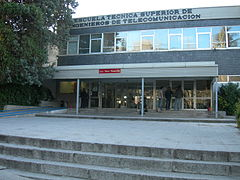
\includegraphics[width=.55\textwidth]{UPM-ETSIT--Sanz_Mancebo} }
	\caption{Figure 1}%
	\label{fig:figure1}
\end{figure}
Example of two figures:
\begin{figure}[h!]
	\centering
	\subfloat[Subtitle 1]{{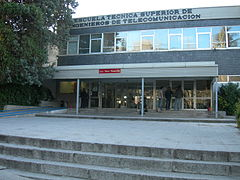
\includegraphics[width=.45\textwidth]{UPM-ETSIT--Sanz_Mancebo} }} \label{fig:subfigure1}
	\qquad
	\subfloat[Subtitle 2]{{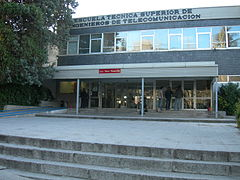
\includegraphics[width=.45\textwidth]{UPM-ETSIT--Sanz_Mancebo} }} \label{fig:subfigure2}
	\caption{Figure 2}%
	\label{fig:figure2}
\end{figure}

Example of table:
\begin{table}[H]
	\begin{center} {\footnotesize
			\begin{tabularx}{\textwidth}{@{} lXlX @{} }
				\multicolumn{2}{c}{} \\ 
				\hline
				
				\normalsize \textbf{Label} & \normalsize \textbf{values} \\

				\hline
				& \\
				label  & Description\\
				& \\
				label  & Description\\
				\hline
		\end{tabularx}}
	\end{center}
	\caption{\footnotesize Table 1}
	\label{table1}
\end{table}

\section{Example of section}
Example of list:
\renewcommand\labelitemi{\ding{117}}
\begin{itemize}
	\item First.
	\item Secondly.
	\item In the third place.
	\item Chapter 4.
	\item Last but not least.

\end{itemize}

%--------------CHAPTER 2-------------------%
\setcounter{chapter}{1}
\chapter{PREVIOUS WORK} \label{previousWork}

\section{Section Example}

\begin{table}[H]
	\begin{center} {\footnotesize
			\begin{tabular}{ccc}
		\hline 
		\textbf{Index} & \textbf{Columns }\\
		\hline
		\rowcolor{blue!20}0 & Blue  \\
		\rowcolor{black!0}1 & White  \\
		\rowcolor{blue!20}0 & Blue  \\
		\rowcolor{black!0}1 & White  \\
		

\end{tabular}}
\end{center}
\caption{\footnotesize Fancy Table}
\label{fancyTable}
\end{table}

Example:

\textbf{\centerline{
$\bigl[ \begin{matrix}
N^{\circ} Examples,  & N^{\circ} Examples, & Example\\
\end{matrix} \bigr]$}}

\section{Section example }
Paragraph
\begin{itemize}
	\item List 1 with image 

\begin{figure}[H]
	\centering
	{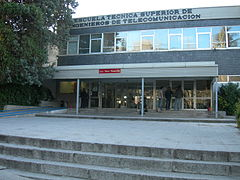
\includegraphics[width=.95\textwidth,height=0.25\textheight]{UPM-ETSIT--Sanz_Mancebo} }
	\caption{Image within a list}%
	\label{fig:image in a list}
\end{figure}


\end{itemize}

\section{Icon Section \protect\icon{android}}\label{sec:iconsection}

\subsection{Subsection example}
Paragraph...

%--------------CHAPTER 3-------------------%

\setcounter{chapter}{2} 



\chapter{STATE-OF-THE-ART}\label{ch:state}
Example of table:
\begin{table}[h]
	\begin{center} {\footnotesize
			\begin{tabular}{llll}
				\hline
				\multicolumn{1}{c}{}   & \multicolumn{1}{c}{\textbf{Label1}} & \multicolumn{1}{c}{\textbf{Label2}} & 
				\multicolumn{1}{c}{\textbf{Label3}} \\
				\hline
				\multicolumn{1}{c}{} & \multicolumn{1}{c}{}& \multicolumn{1}{c}{\textit{Subtitle1}}&\multicolumn{1}{c}{}\\
				\multicolumn{1}{c}{} & \multicolumn{1}{c}{}& \multicolumn{1}{c}{}&\multicolumn{1}{c}{}\\
				\multicolumn{1}{c}{\textbf{Item1 ($\%$)}} & \multicolumn{1}{c}{00.00}     & \multicolumn{1}{c}{00.00}         & \multicolumn{1}{c}{00.00}    \\
				
				
				\multicolumn{1}{c}{} & \multicolumn{1}{c}{}& \multicolumn{1}{c}{\textit{Subtitle2}}&\multicolumn{1}{c}{}\\
				\multicolumn{1}{c}{} & \multicolumn{1}{c}{}& \multicolumn{1}{c}{}&\multicolumn{1}{c}{}\\
				\multicolumn{1}{c}{\textbf{Item2 ($\%$)}} & \multicolumn{1}{c}{00.00}     & \multicolumn{1}{c}{00.00}         & \multicolumn{1}{c}{00.00}    \\
		\end{tabular}}   
	\end{center}
	\caption{\footnotesize Complete Table}	\label{hybridTable}
\end{table}


	
%--------------CHAPTER 4-------------------%


\setcounter{chapter}{3}
\chapter{PROPOSED METHOD} \label{proposal}
Example of pseudocode:  

\begin{algorithmic}[H]
	
	\State $x \gets \textcolor{MidnightBlue}{\begin{matrix} y \\\end{matrix}} $	
	\Repeat $\hspace{0.1cm} items$
	\For{$\hspace{0.31cm} until \hspace{0.31cm}last\hspace{0.21cm} item$} 
	
	\State $x \gets \textcolor{MidnightBlue}{\begin{matrix} y \\\end{matrix}} $	 \newline
	\textcolor{blue!80}{$\hspace{1.45cm}$Some part} 
	
		\State $x \gets \textcolor{MidnightBlue}{\begin{matrix} y \\\end{matrix}} $	
	 \EndFor
	
	 \Until{$ \hspace{0.215cm}100\% accuracy$} 	\Comment{$Assure \hspace{0.21cm}not\hspace{0.21cm} failures$}
	
\end{algorithmic}

%\input{4_Prooposal/result}


%--------------CHAPTER 5-------------------%
\setcounter{chapter}{4}
\chapter{CONCLUSIONS AND FUTURE WORK}
\newpage
\section{Conclusions}

% FUTURE LINES 
\section{Future lines}

$\sbullet[.75] \hspace{0.215cm} $ \textbf{Bullet 1. }

$\sbullet[.75] \hspace{0.215cm} $ \textbf{Bullet 2. }



%-------------------HEADERS---------------%
\pagestyle{plain}
\rhead{}
\lhead{}

\nocite{*}
\bibliographystyle{unsrt} 
\bibliography{6_references/references} \label{ch:Bibliography}


\clearpage
\pagenumbering{alph} 
%--------------ANEXO-------------------%

\chapter*{Annex}
\section*{Python code}\label{anexo1}
\begin{lstlisting}[language=Python]

import numpy as np

def compute_sum(a,b):
	c = a+b
	return c

\end{lstlisting}


\end{document}
%---------------------------------------------------------------------------%

